\chapter{Introduction}\label{ch:introduction}

In the digital age written text has become ubiquitous. % (TODO: cite?)
% TODO: Examples for important written text: Websites, Online Messages like E-Mails, Newspapers, Government Authorities (distribute Information)

Today the ability to comprehend text is a necessary prerequisite to actively participate in society. % nowadays
This poses a challenge to people with communication impairments~\autocite{easyLanguageBook}.
In Germany about 12\% of the population has difficulties to understand and write standard german because of reduced literacy~\autocite{schomacker2023data}.
Complicated texts can act as a barrier which prevents these people from taking part in everyday life~\autocite{easyLanguageBook}
% could lead to exclusion,

Several attempts have been made to create a type of written language that is more comprehensible and accessible.
The primary goal of such languages is to improve communication for a broad range of people with limited reading and writing skills.
This group includes people with communication impairments, people with dementia, language learners, \gls{illit} and older people with visual impairments~\autocite{easyLanguageBook}.

In German two simplified language have gained popularity in recent years: \enquote{Easy Language} and \enquote{Plain Language}.

%The simplified language has to be simple enough to be understood by everyone.
%At the same time it should not be impractical for people that are proficient in standard language.


\section{Easy Language}\label{sec:el}

\gls{el} is a type of simplified language that is regulated by a set of rules.
There are multiple guidelines published by different organizations that define those rules.
The most commonly used guideline is distributed by the \enquote{\gls{nls}}~\autocite{netzwerkLS, easyLanguageBook}.

The \gls{nls} was founded in 2006 and became an official association in 2013~\autocite{netzwerkHistory}.
The association aims to popularize and standardize \gls{el} in Germany.
All members are volunteers~\autocite{netzwerkGoals}.
Among others, the \gls{nls} includes the following people in their target group:
\begin{itemize}[noitemsep]
    \item people with learning difficulties
    \item people with the illness dementia
    \item people that are not proficient in German
    \item people with reduced reading abilities
\end{itemize}
The \gls{nls} intends that texts written in \gls{el} are verified by certified examiners.
Examiners are trained at the \gls{nls} and are usually people in the target group~\autocite{netzwerkPruef}.

\subsection{Rules and Recommendations}\label{subsec:el-rules}
The rules for \gls{el} fall into the categories \enquote{Words}, \enquote{Numbers and Symbols}, \enquote{Sentences}, \enquote{Content} and \enquote{Presentation and Images}.

Words are supposed to be simple.
Technical and foreign words should be avoided.
If difficult words are unavoidable, they have to be explained.
Once a word was introduced to describe a subject, that word should be used again when the subject is referred to.

\begin{figure}[htb]
    \begin{center}
        \colorbox{badred!20}{
            \begin{minipage}{0.6\textwidth}
                \fontfamily{pag}
                A car drove past me.\\
                It was very fast.\\
                The vehicle was red.
            \end{minipage}
        }
        \colorbox{goodgreen!20}{
            \begin{minipage}{0.6\textwidth}
                \fontfamily{pag}
                A car drove past me.\\
                It was very fast.\\
                The car was red.
            \end{minipage}
        }
    \end{center}
    \caption[Using the same word to refer to the same subject.]{Using the same word to refer to the same subject (bottom). Using synonyms can be confusing (top).}
    \label{fig:subject_ref}
\end{figure}
Shorter words are preferred over longer words.
If long words are necessary they should be split with a hyphen character (e.g.\ \enquote{Bundes-Gleichstellungs-Gesetz} instead of \enquote{Bundesgleichstellungsgesetz}).
Additional rules for words are
\begin{itemize}[noitemsep]
    \item the avoidance of acronyms
    \item the use of active voice over passive voice
    \item avoidance of genitive and conjunctive
    \item reduced use of negation
\end{itemize}
Numbers and symbols are another aspect that is addressed by the \gls{nls}-guideline.
Numbers should be written in arabic numerals.
For many people digits are easier to read than the spelled out word (e.g.\ \enquote{5 horses} instead of \enquote{five horses}).#
Thus, smaller numbers are to be witten in digits.
Very large numbers are replaced by rough estimations (e.g.\ \enquote{Many People} instead of \enquote{14.795 People}).
The same goes for percentages.
If unusual symbols (e.g.\ §) are used they need to be explained.

The structure of sentences has a big impact on readability. % TODO: quelle?
In \gls{el} sentences are supposed to be short.
Every sentence should only include one statement.
After each sentence a new line is started.
Sentences with simple structures like \enquote{subject, verb, object} are preferred.
More complex sentences should be broken up in smaller pieces.
These smaller pieces do not necessarily need to form a complete sentence.
\begin{figure}[htb]
    \begin{center}
        \colorbox{badred!20}{
            \begin{minipage}{0.6\textwidth}
                \fontfamily{pag}
                Do you want to go swimming or watch a movie?
            \end{minipage}
        }
        \colorbox{goodgreen!20}{
            \begin{minipage}{0.6\textwidth}
                \fontfamily{pag}
                Do you want to go swimming? \\
                Or watch a movie?
            \end{minipage}
        }
    \end{center}
    \caption[Splitting longer sentences in \glsentrylong{el}.]{Splitting longer sentences in \glsentrylong{el}. To comply with the rules of \gls{el} the (top) sentence is split in two. The second part of the (bottom) example does not form a complete sentence on its own.}
    \label{fig:split_sentence}
\end{figure}
%\begin{mybox}{Bad example}
%    Do you want to go swimming? \\
%    Or watch a movie?
%\end{mybox}
Sentences with subordinate clauses can be broken up similarly.

Topics should not be distributed across the text.
Related content should be kept together.
References to other texts are to be avoided.
In the translation process from standard German to \gls{el} content can be omitted if necessary.
Likewise, additional content can be added to make the text more understandable.

The presentation of text is another aspect that impacts clarity and readability.
The \gls{el}-guideline recommends to use a big font size and big line spacing.
Furthermore, text is to be left-aligned.
Backgrounds are supposed to be in light color while the written text is colored darkly.
Text should be structured in many paragraphs with frequent headlines.
Using bullet points instead of comma separated enumerations improves clarity.
Images can be added to accompany the text~\autocite{netzwerkLS}.

\subsection{Prevalence and Adoption of Easy Language}\label{subsec:el-adop}

\glsentrylong{el} contains features that go against standard german.
The unique layout with very short lines makes it easy to recognize texts in \gls{el}.
This helps the target group to find texts written in \gls{el} easily.
But the strong divergence from standard German has been repeatedly criticised.
In 2015 the Federal State Parliament of Schleswig-Holstein passed a law to make elections more accessible.
Information regarding elections was sent out to all voters in \gls{el}.
This sparked outrage in the population and was denounced by multiple politicians.
As a result the passed law was reverted~\autocite{easyLanguageBook}.

While \gls{el} has yet to find acceptance in the general population, it has already been incorporated into german law.
In 2002 the \gls{bgg} was adopted.
The \gls{bgg} guarantees equal living conditions to people regardless of disabilities.
In 2018 the \gls{bgg} was extended to include clearer instructions for accessibility~\autocite{bggInfo}.
Since then public authorities have to provide information in \gls{el} as specified in section 2, paragraph 11~\autocite{bgg2018}.
Today \gls{el} can be found on many websites of government departments and municipal institutions (e.g.\ the City Cologne: \url{https://www.stadt-koeln.de/artikel/07808/index.html}).

\begin{figure}
    \centering
    \colorbox{goodgreen!20}{
        \begin{minipage}{0.6\textwidth}
            Fische sind Tiere. \\
            Sie leben im Wasser. \\
            In Flüssen, im Meer und in Seen. \\
            \\
            Fische atmen durch Kiemen. \\
            Das ist ein Körper-teil. \\
            Dadurch können sie unter Wasser atmen.
        \end{minipage}
    }
    \caption[Text written in \glsentrylong{el}.]{Text written in \gls{el} taken from the online dictionary \enquote{Hurraki} (\url{https://hurraki.de/wiki/Fische}).}
    \label{fig:easy_text}
\end{figure}


\section{Plain Language}\label{sec:pl}
% TODO: Überarbeiten, abschnitt ist seltsam
\gls{pl} is a simplified language that is much closer to standard language.
Originally, it was not intended for people with disabilities.
\gls{pl} is often used to explain domain specific texts in expert language to less informed people.
Moreover, it addresses language learners e.g.\ migrants and people that learn German as a second language~\autocite{easyLanguageBook}.

In the English language guidelines for \gls{pl} have existed for a long time.
Some early works on more accessible language were published in the beginning of the 20th century.
From the 1960s on the US government pushed to propagate the use of \gls{pl}.
The goal was to improve communication between citizens and experts from administrative institutions.
Several instruction manuals for \gls{pl} were distributed.
Since 2010 federal agencies in the US are required to offer information in a form that is well understood by the citizens.

In Germany efforts for \gls{pl} have only been made very recently.
In the 1980s \enquote{Bürgernahe Sprache} (in English: \enquote{language that is close to the citizens}) was created to make administrative texts more comprehensible.
\enquote{Bürgernahe Sprache} does not take people with communication impairments and less educated people into account.
Thus, it does not satisfy all expected conditions of a simplified language.
In the 2000s multiple approaches for \gls{pl} with a broader target groups were attempted.
But none of them have been widely accepted as a standard yet.
Typical features of \gls{pl} are
\begin{itemize}[noitemsep]
    \item use of common words
    \item use of short words
    \item avoidance of ambiguous words
    \item precise formulations
    \item short sentences
    \item active voice
    \item clear sentence structure (e.g.\ a maximum of two subordinate clauses)
    \item avoidance of acronyms
\end{itemize}
These directives are similar to some of the rules in the \gls{el}-guideline.
But \gls{pl} does not break any rules of standard German.
That might be a reason why \gls{pl} is generally viewed in a more positive light than \gls{el} by many people. % viewed favorably
Moreover, \gls{pl} can be more flexible and less restrictive as there are no fixed rules.
Writers of \gls{pl} are supposed to factor in the audience of the text and make changes accordingly~\autocite{easyLanguageBook}.

\begin{figure}
    \centering
    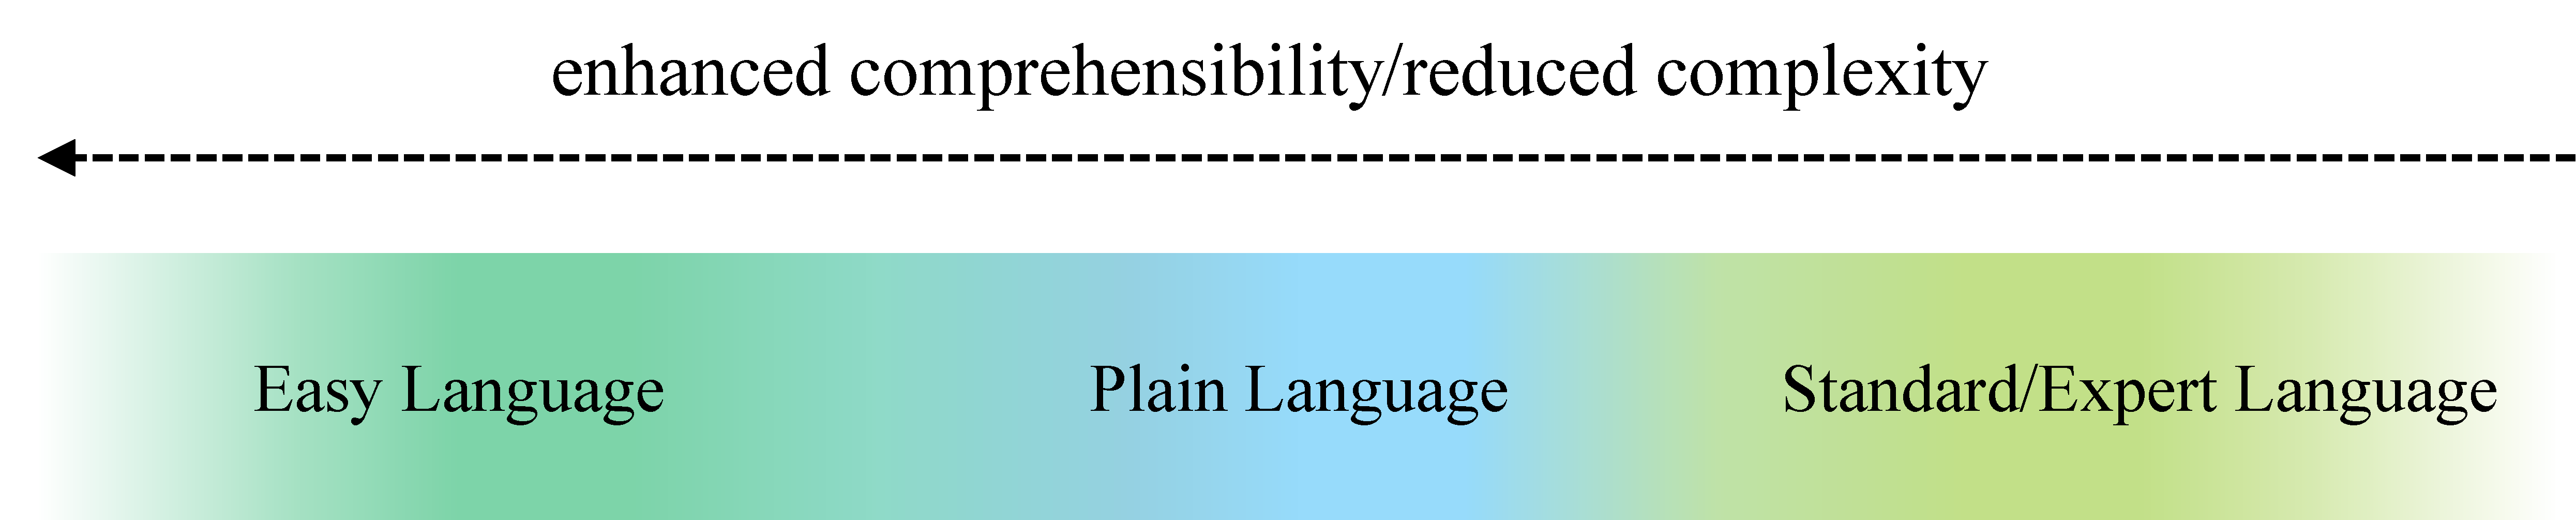
\includegraphics[width=\linewidth]{images/easy_languages}
    \caption[Different levels of text complexity and comprehensibility.]{Different levels of text complexity and comprehensibility. The different types of languages overlap in certain aspects~\autocite{easyLanguageBook, selbsterstellt}}
    \label{fig:languages}
\end{figure}


%\section{Terminologie}\label{sec:term}

%ambiguity of terminology

%    more difficult to understand than easy language
%
%
%From~\autocite{un2008}:
%Article 9 -Accessibility: "sinage in easy to read and understand forms", "ensure access to information"
%
%Article 2: plain-language listed under communication
%
%Article 29 - Participation in political and public life

%easy, plain, simple with very similar meanings

%    different guidelines:
%        inclusion europe
%        Netzwerk Leichte Sprache -> most commonly used
%        Barrierefreie-Informationstechnik-Verordnung (BITV 2.0)
%
%    rulebooks published by Duden


%

%From~\autocite{schomacker2023data}:
%"Easy language is roughly equivalent with level A2 of the Common European Framework of Reference for Languages (CEFR)"


\section{Automatic Language Simplification}\label{sec:langSimp}

Writing texts in \gls{pl} or \gls{el} and translating complex texts into simpler forms requires much effort~\autocite{easyLanguageBook}.
Hence, there is a demand for tools that can assist in this process.
In the context of \gls{nlp} the task of computer aided reduction of text complexity is known as \gls{ats}~\autocite{Ansch_tz_2023}.
\gls{ats} is similar to other \gls{nlp}-tasks like summarization~\autocite{rios-etal-2021-new} and language translation~\autocite{aumiller2022klexikon}.
It is a sequence-to-sequence (seq2seq) task~\autocite{Ansch_tz_2023}.
% meaning the input and output spaces consist of sequences of varying length
The goal of \gls{ats} is to create a system that takes a text in standard or expert language as an input and outputs a simplified version of that text.

\gls{ats} is a relatively new machine translation task~\autocite{schomacker2023data}.
Especially simplification of German text has not seen a lot of research~\autocite{Ansch_tz_2023}.

An early rule-based approach for language simplification was presented by~\autocite{suter2016}

In translation solutions based on Deep Learning are generally superior to rule-based methods.
Though, they require vast amounts of Data.~\autocite{otter2019survey}

From~\autocite{klöser2024german}:


From~\autocite{Ansch_tz_2023}:

From~\autocite{aumiller2022klexikon}:

From~\autocite{toborek2023new}:

From~\autocite{sauberli-etal-2020-benchmarking}

From~\autocite{battisti-etal-2020-corpus}

From~\autocite{madina2023easytoread}

From~\autocite{schomacker2023data}:
text simplification with machine learning is still very new compared to other translation tasks

From~\autocite{rios-etal-2021-new}: 20min Dataset









